\documentclass[12pt,draftcls,onecolumn]{IEEEtran}
%\documentclass[onecolumn]{IEEEtran}

\usepackage{amsmath}
\usepackage{amsthm}
\usepackage{amssymb}  % assumes amsmath package installed
%\usepackage{algorithmic}
%\usepackage{algorithm}
\usepackage{algorithm}
\usepackage{algpseudocode}
\usepackage{algpseudocode}

\algnewcommand{\algorithmicand}{\textbf{ and }}
\algnewcommand{\algorithmicor}{\textbf{ or }}
\algnewcommand{\OR}{\algorithmicor}
\algnewcommand{\AND}{\algorithmicand}
\algnewcommand{\var}{\texttt}

\usepackage{cite}
\usepackage{color}
\usepackage{comment}
\usepackage{epsfig}
\usepackage{float}
\usepackage{graphicx}
\usepackage{multicol}
\usepackage{subfigure}
\usepackage{setspace}
\usepackage{comment}
\usepackage{subfig} % for subfigures
\usepackage{caption}

%\usepackage[linesnumbered,ruled]{algorithm2e}

\usepackage[none]{hyphenat}

\newtheorem{theorem}{Theorem}[section]
\newtheorem{lemma}[theorem]{Lemma}
\newtheorem{proposition}[theorem]{Proposition}
\newtheorem{corollary}[theorem]{Corollary}
\newtheorem{remark}[theorem]{remark}

\begin{document}

\title{Path Planning of Webot Satisficing Experiment ---- Workspace and C-Target Construction, Off-line EER Calulation and Milestones Generation }


\author{  Min Zheng \\  \today}

\date{\today}

% make the title area
\maketitle


%\IEEEpeerreviewmaketitle

%%%%%%%%%%%%%%%%%%%%%%%%%%%%%%%%%%%%%%%%%%%%%%%%%%%%%%%%%%%%%%%%%%%%%%%%%%%%%%
This project considers the integrated navigation and control of an unmanned ground vehicle(UGV) deployed to visually classify multiple targets in an obstacle-populated environment. 
This report includes the problem setup and the contruction of the $\mathcal{C}_{Target}$ . Then the Exptected Entropy Reduction (EER) method is applied in addition to a hybrid sampling method to obtain milestones for the roadmap. 

\section{Workspace construction} 

The workspace is the same as the one used for active satisficing human studies. 
The UGV and 30 target objects are in the same environment that consists of four rooms, denoted as the region-of-interest (ROI).
Similar to the human studies, there are 30 targets, denoted as $\mathcal{T} = \{\mathcal{T}_i; i = 1,2,...30; \mathcal{T} \subset W \}$.
The targets are considered as points.
A two-dimensional representation from the webot environment was extracted, and the workspace is constructed in MatLab, as shown in the figure below  (Figure \ref{fig:2}). 


The construction of workspace is built in an object oriented manner with classes of obstacles, targets and robot, each has properties and functionalities.  
Note that the table and the chairs are treated differently from other obstacles.
Since their top surfaces are higher than the robot, only their legs will be considered as obstacles. 


\begin{figure}[p]
\centering
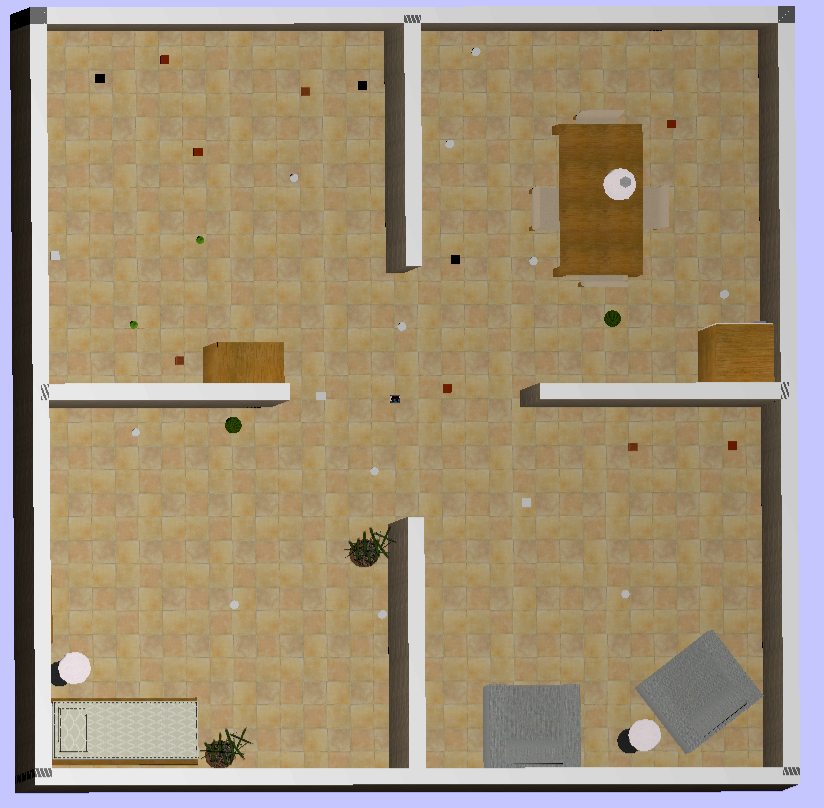
\includegraphics[width=10cm]{figures/webotTop}
  \caption{Top view of the webot environment}
  \label{fig:1}
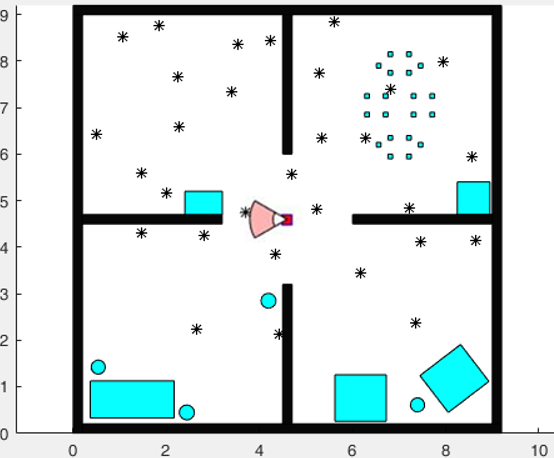
\includegraphics[width=13cm]{figures/newWorld}
  \caption{2D representation built in MatLab. Obstacles are represented by colored regions, and targets represented by the stars. The UGV is  the red square, while its FOV is the red area within the fan shape.}
  \label{fig:2}
\end{figure}



\clearpage


%%%%%%%%%%%%%%%%%%%%%%%%%%%%%%%%%%%%%%%%%%%%%%%%%%%%%%%%%%%%%%%%%%%%%%%%%%%%%%
\section{UGV's specs and FOV} 


The UGV sensor in the webot environment has platform geometry $\mathcal{A}$, and FOV geometry $S \subset \mathbb{R}^2 $. 
The dimension of UGV is 0.12m x 0.10m in 2D.
Its translation step is 0.01m, and rotation step is $\pi/12 \; rad$, which are the minimum possible steps the robot can perform in translation and rotation. 
The UGV configuration is described in  (Figure \ref{fig:1}).
The configuration vector is defined as $q \equiv [x  \quad  y  \quad  \theta]^T$.



In order to combine with Zeyu's visual classification project, the FOV was determined based on requirement of  images processing algorithm. 
Successful image processing and cue classification requires the image to be taken within a minimum and a maximum distance, denoted by $d_{min}$ and  $d_{max}$. 
In human tests, the open angle of FOV for the on board camera is $\alpha =\pi/4  \;rad $. 
Therefore the same  $\alpha$ is used here.
The  images processing algorithm requires a minimum distance from the target.
If the UGV is too close from the target, the camera is not able to capture a full image of the target object. 
Meanwhile, in the human tests software setup, the robot must be within 1m from the target to  measure or classify.
In such manner, the range of distance from target is conservatively set within $d_{min} = 0.3 \;m$ and  $d_{max}=0.8\; m$.
In order to better work with the image processing algorithm, these parameters, especially $d_{max}$ may be subject to changes due to the highly sensitive manner of the algorithm. 
For example, it may be affected by whether the algorithm allows multiple objects to appear in the view. 

\begin{figure}
 \centering
  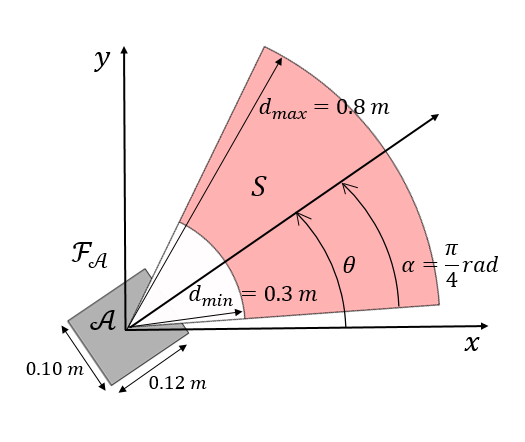
\includegraphics[width=8cm]{figures/FOV}
  \caption{Configuration and FOV of the UGV.}
  \label{fig:3}
\end{figure}


\clearpage






%%%%%%%%%%%%%%%%%%%%%%%%%%%%%%%%%%%%%%%%%%%%%%%%%%%%%%%%%%%%%%%%%%%%%%%%%%%%%%
\section{Free Configuration Space, $\mathcal{C}_{free}$} 


Assume that the UGV can freely rotate. Thus  $ \alpha  \in (-\pi $ , $\pi) $.
In x-y plane, a location is defined to be in $\mathcal{C}_{free}$ if the UGV can freely rotate around its center, which is at the given location.
The locations where some subsets of all possible $ \alpha$ are be allowed is discarded from $\mathcal{C}_{free}$, considering the problem of getting stuck. 
Given the geometry of the UGV, it requires that the bounding circle of the UGV (Figure \ref{fig:3}) does not intersect with any obstacles.
The result $\mathcal{C}_{free}$ is shown in Figure \ref{fig:6}.

\begin{figure}
 \centering
  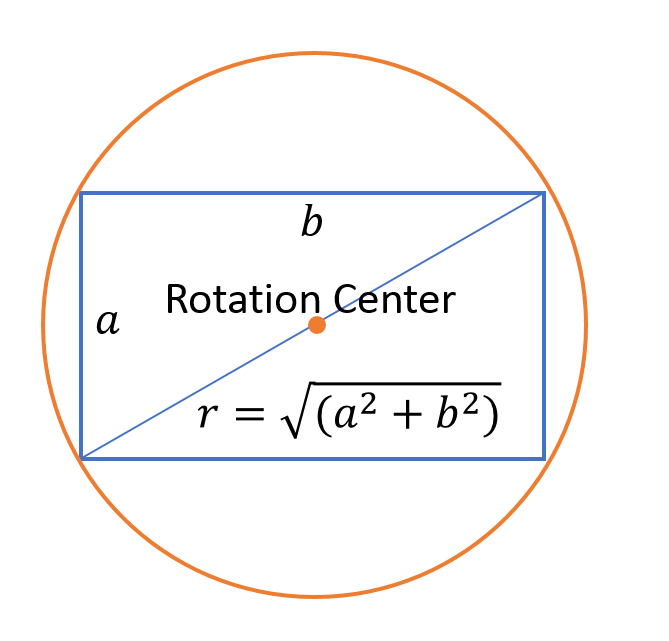
\includegraphics[width=8cm]{figures/rot_demo}
  \caption{The area(orange circle) swept by rotating $\mathcal{A}$ (blue rectangle) around  its center. }
  \label{fig:4}
\end{figure}

\begin{figure*}[htp]
  \centering
  \subfigure[ $\mathcal{C}_{free}$ for the whole world map]{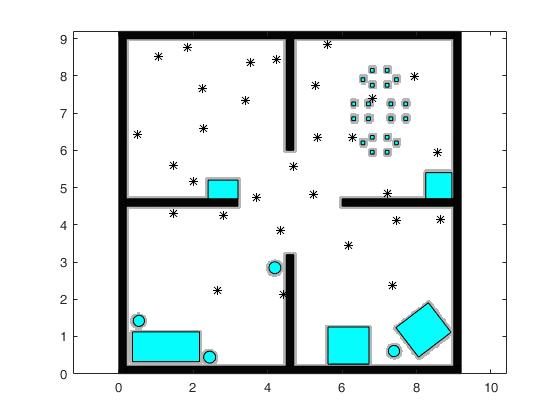
\includegraphics[width=12cm]{figures/Cfree}}\quad
  \subfigure[zoomed-in demonstration of $\mathcal{C}_{free}$, where the center of the circle represents the UGV center location, so that the ]{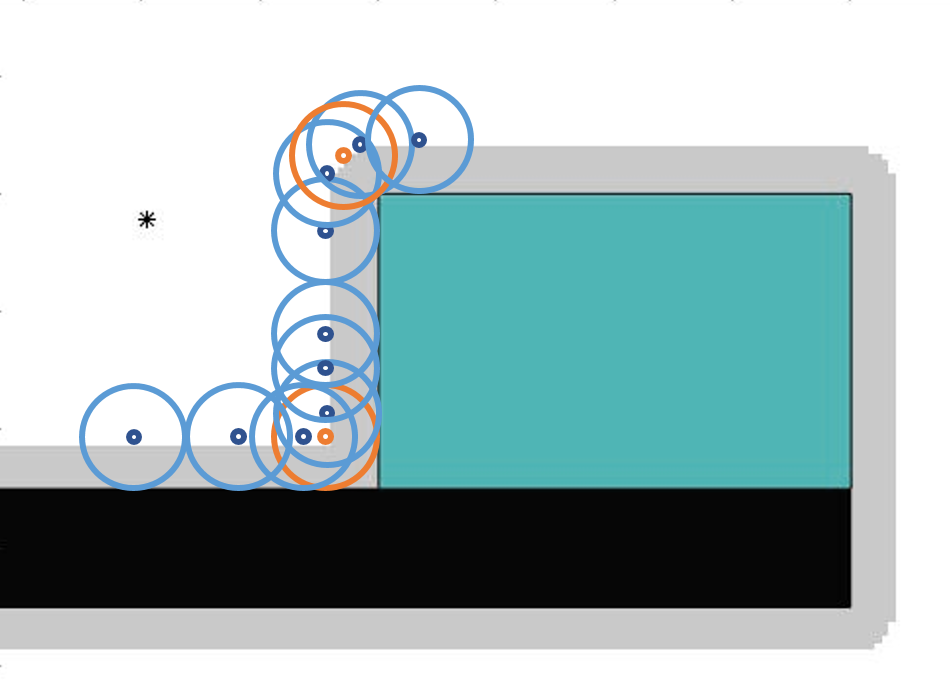
\includegraphics[width=8cm]{figures/Cfree_demo1}}
  \caption{ $\mathcal{C}_{free}$  of the given world map denoted by white region. Grey area is not in  $\mathcal{C}_{free}$ }
  \label{fig:6}
\end{figure*}


\clearpage


%%%%%%%%%%%%%%%%%%%%%%%%%%%%%%%%%%%%%%%%%%%%%%%%%%%%%%%%%%%%%%%%%%%%%%%%%%%%%%
\section{Mapping Targets into Robot Configuration Space} 


Assume that the UGV camera is mounted at the center the UGV and always face the same direction as the UGV.
$\mathcal{C}_{Target}$  is defined so that the target $\mathcal{T}_i$ in $\mathcal{W}$ maps  in the robot's configuration space  $\mathcal{C}_{free}$ to the C-target region  $\mathcal{CT}_i = \{q \in \mathcal{C}_{free}    |    \mathcal{S}(q) \cap \mathcal{T}_i  \neq  \emptyset \}$.
A simple $x-y$ plane demonstration (Figure \ref{fig:4}) demonstrates the effect of the distance to the target.
In (a), the robot is within $\mathcal{C}_{Target}$, since the target is in the robot's FOV when it faces $-\pi/2 \: rad$.
In (b), the robot is not in $\mathcal{C}_{Target}$, and it can not detect the target no matter how it rotates at its current position. 


Line-of-sight visibility is taken into account as well, as obstacles in the line of sight may cause occlusions with respect to the target of interest. 
As shown in Figure \ref{fig:5}, let the camera state $\mathbf{x}$ demote the position of FOV apex ($\mathcal{O}_{A}$) in inertial frame  $\mathcal{F}_{W}$, and the target state  $\mathbf{x}_{T}$ demote the inertial position of the point target $\mathcal{T}$. 
The relative position of  $\mathcal{T}$ with respect to the camera  $\mathcal{F}_{A}$ is $\mathbf{r}_{T} = (\mathbf{x}_{T} - \mathbf{x})$.
Then, $\mathbf{x}_{T}$ thus also the target $\mathcal{T}$ is the in the line of sight of the camera at $\mathbf{x}$ if there are no points in the obstacle region $\mathcal{B}$ that are co-directional with  $\mathbf{r}_{T}$ and closer to $\mathbf{x}$ than $\mathbf{x}_{T}$. 
For implementation, the test checks if $\mathbf{r}_{T}$ intersects with $\mathcal{B}$.
An example in the workspace is shown in Figure \ref{fig:7}.


The algorithm iterates through every configuration in $\mathcal{C}_{free}$.
At each configuration, it checks if there exists any target in the FOV that passes the line-of-sight test.
If there exists such target, this configuration is in $\mathcal{C}_{Target}$.
A zoom-in example for the 3-D configuration is shown in (Figure \ref{fig:8}).
Then the $\mathcal{C}_{Target}$ for the workspace is shown (Figure \ref{fig:9} and Figure \ref{fig:12}).



\begin{figure*}[htp]
  \centering
  \subfigure[$q \in \mathcal{C}_{Target}$]{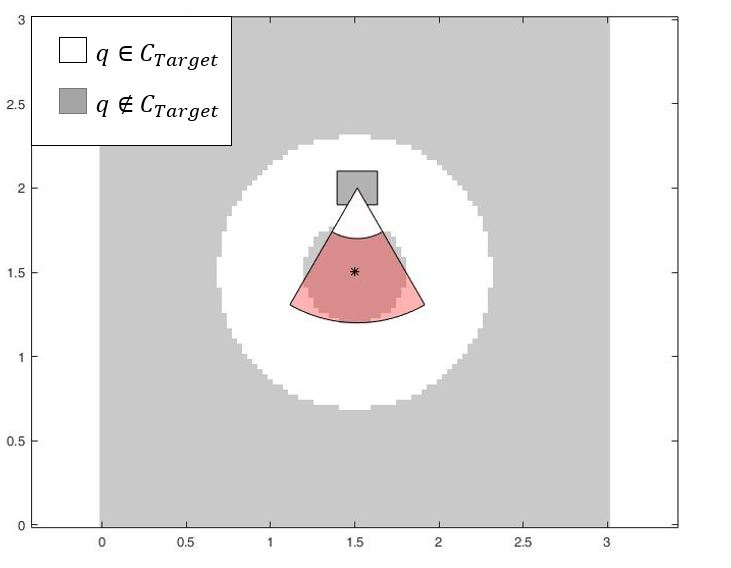
\includegraphics[width=9cm]{figures/oneTargetTrue}}\quad
  \subfigure[$q \not\in  \mathcal{C}_{Target}$]{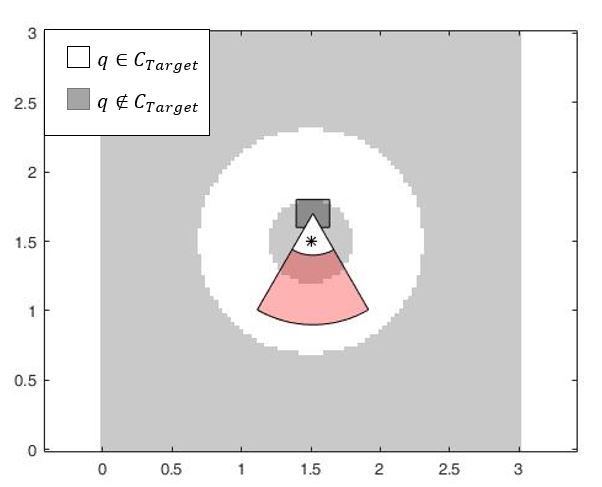
\includegraphics[width=9cm]{figures/oneTargetFalse}}
  \caption{Example of C-target with one target. C-target denoted by white area, and the star denotes the target. The target must fall in the red region (robot FOV) to be classified or measured. In both examples, the robot is facing $\theta = -\pi/2 \; rad$}
  \label{fig:4}
\end{figure*}


\begin{figure}
 \centering
  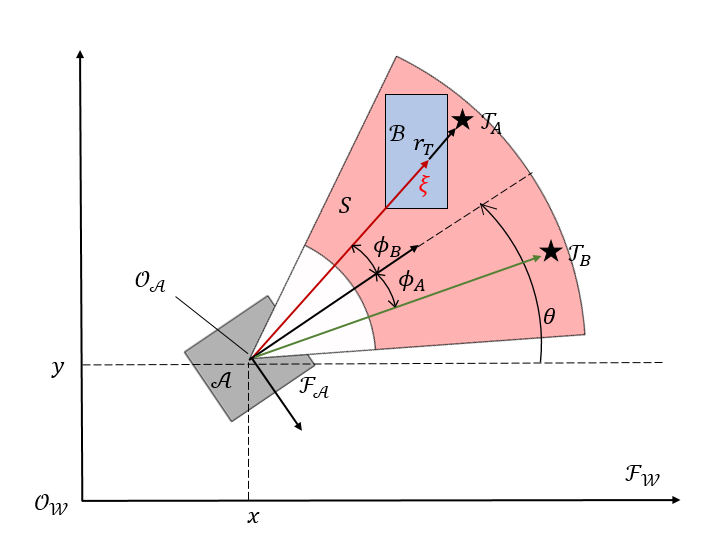
\includegraphics[width=12cm]{figures/lineSight}
  \caption{With the FOV, $\mathcal{S}$ introduced in Figure \ref{fig:3}, a line-of-sight visibility test is demonstrated for two targets  $\mathcal{T}_{A}$  and $\mathcal{T}_{B}$ in $\mathcal{S}$.  $\mathcal{T}_{A}$  is occluded by obstacle  $\mathcal{B}$  because there exists at least a point,  $\xi$ ,  in  $\mathcal{B}$ that fails the line-of-sight test. And $\mathcal{T}_{B}$ is not occluded by obstacles since there is no such $\xi$.}
  \label{fig:5}
\end{figure}

\begin{figure}
 \centering
  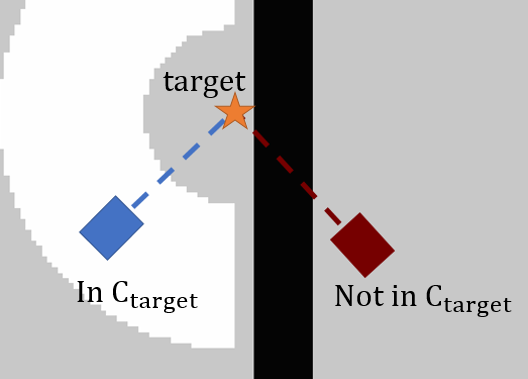
\includegraphics[width=5cm]{figures/visibility_eg}
  \caption{Example of visibility problem handling for a target near the wall. The blue and red rectangles denote two possible UGV configurations. The dashed line denotes the robot forward direction. The blue configuration is in C-Target, but the red is not since its view is blocked by the obstacle.}
  \label{fig:7}
\end{figure}






%\begin{figure}
% \centering
%  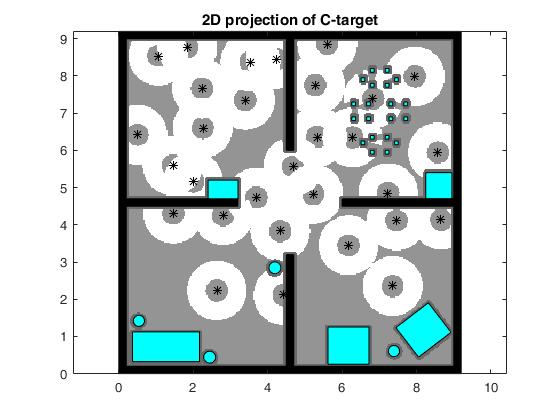
\includegraphics[width=15cm]{figures/CTarget_v2}
%  \caption{x-y projection of C-Target, which is denoted by white.}
%  \label{fig:6}
%\end{figure}


\begin{figure*}[htp]
  \centering
  \subfigure[ perspective view]{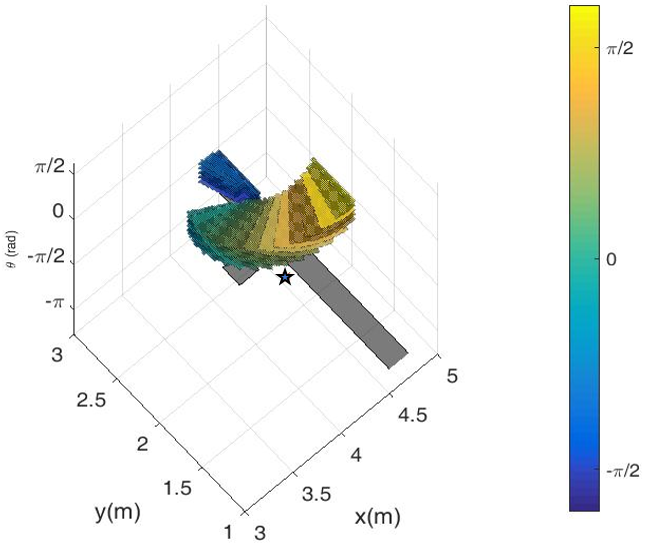
\includegraphics[width=10cm]{figures/ctarget_demo_p}}\quad
  \subfigure[$x-y$  view ]{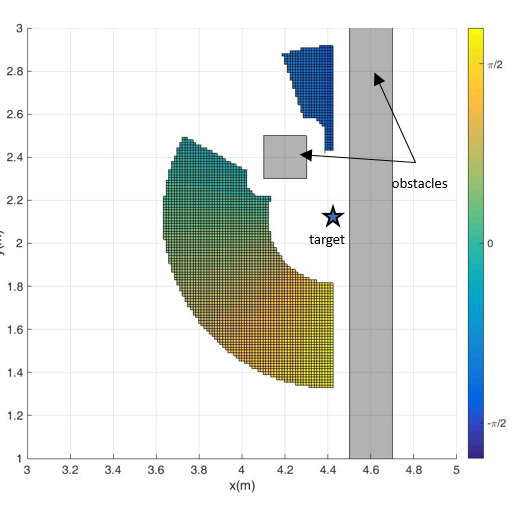
\includegraphics[width=8cm]{figures/ctarget_demo_xy}}\quad
  \subfigure[$x-\theta$  view  and $y-\theta$  view]{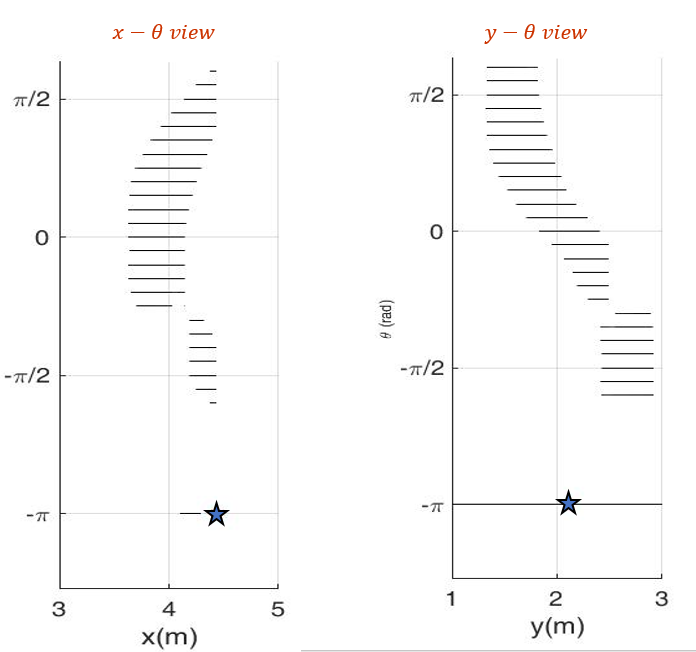
\includegraphics[width=8cm]{figures/ctarget_demo_xytheta}}
  \caption{ An example zoom-in of $\mathcal{C}_{target}$}
  \label{fig:8}
\end{figure*}

\begin{figure*}[htp]
  \centering
  \subfigure[$x-y$  view]{\includegraphics[width=14cm]{figures/ctarget_xy}}
 \subfigure[$x-\theta$  view]{\includegraphics[width=10cm]{figures/ctarget_xtheta}}
  \caption{ $\mathcal{C}_{target}$}
  \label{fig:9}
\end{figure*}


\begin{figure*}[htp]
  \centering
  \subfigure[ ]{\includegraphics[width=13cm]{figures/ctarget_p2}}\quad
  \subfigure[ ]{\includegraphics[width=13cm]{figures/ctarget_p}}\quad
  \caption{ Perspective view of $\mathcal{C}_{target}$}
  \label{fig:12}
\end{figure*}


\clearpage
%%%%%%%%%%%%%%%%%%%%%%%%%%%%%%%%%%%%%%%%%%%%%%%%%%%%%%%%%%%%%%%%%%%%%%%%%%%%%%
\section{Expected Entropy Reduction}



EER method is applied in the milestone generation and the on-line path planning, so that the UGV finds and interacts with the targets motivated by the entropy reduction of revealing a possible feature. 
The target features, Bayesian Network(BN) structure and Conditional Probability Table(CPT) are the same as the one used in human tests as well as visual classification.
The targets have 3 levels of features: shape, color and textures, each is a random variable named $X_{1}$, $X_{2}$ and $X_{3}$.
By the EER calculation(in Report 170724), given the CPTs shown in Table \ref{table.1}, the corresponding EER is shown in  Figure \ref{fig:13} and  Figure \ref{fig:14}.

\begin{table}[!htbp]
\centering
\caption{An example of CPT of the target objects}
\label{table.1}
\begin{tabular}{|l|l|l|l|l|l|l|l|l|} % l = left, r = right, c = center
\hline
Cue & \multicolumn{8}{c|}{P(cue)} \\ \hline % l = left, r = right, c = center
$x_{k1}$ & \multicolumn{4}{c|}{0.43 (sphere)} & \multicolumn{4}{c|}{0.57 (box)} \\ \hline % l = left, r = right, c = center
$x_{k2}$ & \multicolumn{2}{c|}{0.64} & \multicolumn{2}{c|}{0.36} & \multicolumn{2}{c|}{0.69} & \multicolumn{2}{c|}{0.31} \\ \hline % l = left, r = right, c = center
$x_{k3}$ & \multicolumn{1}{c|}{0.69} & \multicolumn{1}{c|}{0.31} & \multicolumn{1}{c|}{0.37} & \multicolumn{1}{c|}{0.63} & \multicolumn{1}{c|}{0.08} & \multicolumn{1}{c|}{0.92} & \multicolumn{1}{c|}{0.21} & \multicolumn{1}{c|}{0.79} \\ \hline
$ID$ & Apple & Watermelon & Orange & Basketball & Cardboard box & Wooden box & Computer & Book \\ \hline
$Z$ &  \multicolumn{1}{c|}{0.9} &  \multicolumn{1}{c|}{0.1} & \multicolumn{1}{c|}{0.9}  & \multicolumn{1}{c|}{0.9}  &\multicolumn{1} {c|}{0.9}  & \multicolumn{1}{c|}{0.9}   &\multicolumn{1}{c|}{0.9}  &\multicolumn{1} {c|}{0.9}   \\ \hline % l = left, r = right, c = center
\end{tabular}
\end{table}
\clearpage


\begin{figure}
 \centering
  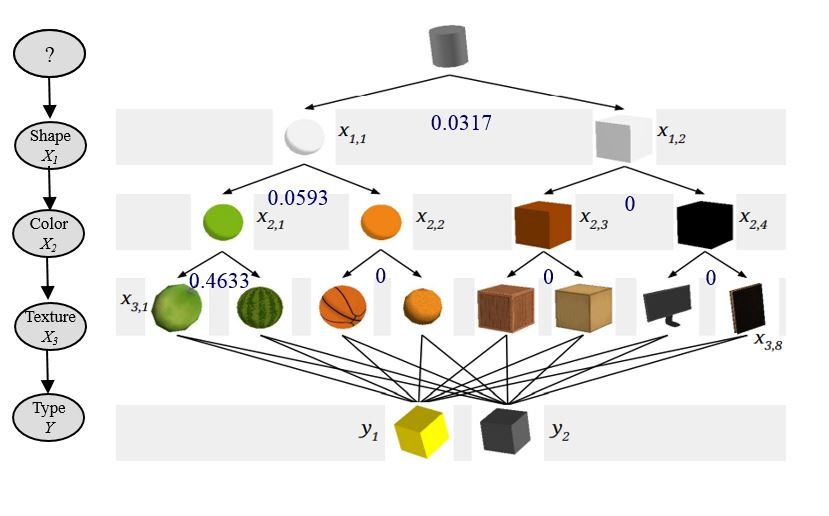
\includegraphics[width=15cm]{figures/oneStepEER}
  \caption{Single-step EER}
  \label{fig:13}
\end{figure}

\begin{figure}
 \centering
  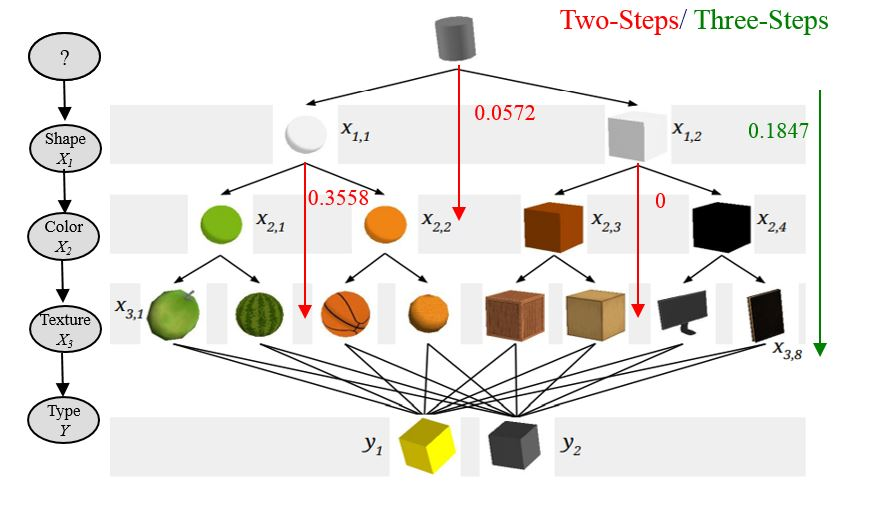
\includegraphics[width=15cm]{figures/someStepEER}
  \caption{Multiple-steps EER}
  \label{fig:14}
\end{figure}


\clearpage
%%%%%%%%%%%%%%%%%%%%%%%%%%%%%%%%%%%%%%%%%%%%%%%%%%%%%%%%%%%%%%%%%%%%%%%%%%%%%%
\section{Milestones Sampling}
 Given the resolution required for the roadmap, the  time complexity and space complexity of Sampling Distribution Generation Algorithm are high.
Therefore a simplified sampling method is proposed (Algorithm 1).
A hybrid strategy is used to combine a bridge test for narrow passages and a uniform probability density function in wide-open regions in order to provide coverage in both.
Let $b$ and $b'$ be two random variables representing the two endpoints of a bridge in $C_{2D}$.
While $C_{2D}$ is configuration in 2D space,  $q \equiv [x  \quad  y  ]^T$.

Since bridges must connect $C_{obstacles}$, $b$ is sampled from a uniform distribution $f(b)$ over $CB$.
And $b'$ is sampled from a multivariate Gaussian PDF that is radially symmetric, with mean at $b$'s location, and a self-defined standard deviation.

%\begin{equation}
%f(b'\; |\; b) = \lambda_{b}(b')I(b')/Z_{b}
%  \label{eq:2}
%  \end{equation}
%Where $/Z_{b}$ is the normalization factor, and 


Let $N_{H}$ denote the total number of milestones generated using hybrid strategy.
We assign a user-defined parameter $0\leq v \leq 1$, which emphasizes either either distribution in the mixture.
So that the $N_{H}$  milestones should be split into  $N_{U} =N_{H}*v $ and $N_{RBB} =N_{H}*(1-v) $, representing uniform and RBB (Randomized Bridge Builder).

As discussed in the Narrow Passage Sampling paper, RBB may generate some milestones near the corner, which is unhelpful.
To reduce the false positives near corner, the orthogonal test is performed for a RBB generated milestone. 
The test draws a line segment orthogonal to the bridge.
The line segment length is a pre-defined variable.
The milestone is accepted if the line segment is collision-free with the $CB$.
 Figure \ref{fig:15} and  Figure \ref{fig:16} demonstrates an example case of using the orthogonal test.


\begin{figure*}[htp]
  \centering
  \subfigure[Example case, the orthogonal test is not used. Some milestones are generated near the corner, which is not helpful.]{\includegraphics[width=12cm]{figures//RBB_woOrthoTest}}\quad
  \subfigure[Example case of applying the orthogonal test ]{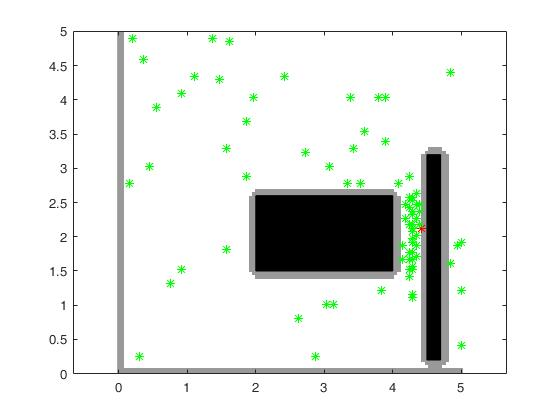
\includegraphics[width=12cm]{figures/RBB_wOrthoTest}}\quad
  \caption{An example case on the orthogonal test}
  \label{fig:15}
\end{figure*}


%\begin{equation}
%\pi_{H} = v\pi_{G}+(1-v)\pi_{U}
%  \label{eq:1}
%  \end{equation}
\begin{algorithm}
   \caption{Simplified Hybrid Sampling Combined with EER}
    \begin{algorithmic}[1]
      \Function{Milestones}{$C$, $C_{free}$}\Comment{Where MS - milestone}
        \State Let $MS_{U}$ and $MS_{RBB}$ be empty arrays
        \While {$N_{U}$ not reached \OR  $N_{RBB}$ not reached}
            \State Uniformly generate a point $q_1$ in $C_{2D}$  
	 \If  {$q_1 \in C_{free}$ \AND $N_{U}$ not reached}
	 \State Record $q_1$ in $MS_{U}$
	 \Else
	  \While {$q_p$ is not a valid RBB milestone}
             \State Generate $q_2$ by multivariate Gaussian PDF
	  \If { $q_2 \in CB$}
	  \State $q_p = (q_1+q_2)/2$	
	  \If {$q_p \in C_{free}$ \AND  Orthogonal Test Passes}
	  \State Record $q_p$ in $MS_{RBB}$
	  \EndIf 	
             \EndIf 
	 \EndWhile	 
	 \EndIf
        \EndWhile
        \For {every $q$  in  $MS_{U}$  and  $MS_{RBB}$ }
        \State Calculate $EER(q)$ 
        \EndFor
      
       \EndFunction
\end{algorithmic}
\end{algorithm}

\clearpage



%\begin{figure}
% \centering
%  \includegraphics[width=12cm]{figures/RBB_woOrthoTest}
%  \caption{}
%  \label{fig:15}
%\end{figure}
%
%\begin{figure}
% \centering
%  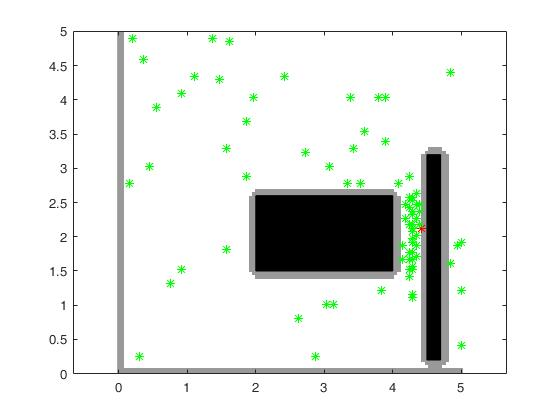
\includegraphics[width=12cm]{figures/RBB_wOrthoTest}
%  \caption{Example case of applying the orthogonal test.}
%  \label{fig:16}
%\end{figure}



When calculating the EER of a given target, if the configuration is in $\mathcal{C}_{Target}$, its EER is the single-step EER of the nearest target if there is cue unrevealed. 
Currently, only single-step EER is considered, because multiple-step EER is rather complex.
 For example, if two targets are both in the FOV, and the nearest one has only one cue to be revealed, the robot may be able to reveal cues of the second target without changing configuration.
A zoom-in example with target A and B (Figure \ref{fig:17}) demonstrates a case with the proposed protocol.
Even though milestone a and b are near A, they are not in the  $\mathcal{C}_{Target}$ region of target A. 
Therefore their EER is the EER of target B.
Milestone c and d are in the $\mathcal{C}_{Target}$ of both A and B. 
Since they are nearer to target A, their EER is that of A.



The milestone generated for the entire road-map is shown in\ref{fig:16}. 
A possible plan is to select, for example 50 milestones that have the highest EER. 
Then another 50 milestones is randomly selected from the rest. 
Meanwhile, the given the 2D configuration of a milestone, the third dimension $\theta$ can be determined either from reading the pre-calculated result or re-calculating by the method in Section $\mathcal{C}_{Target}$.


\begin{figure}
 \centering
  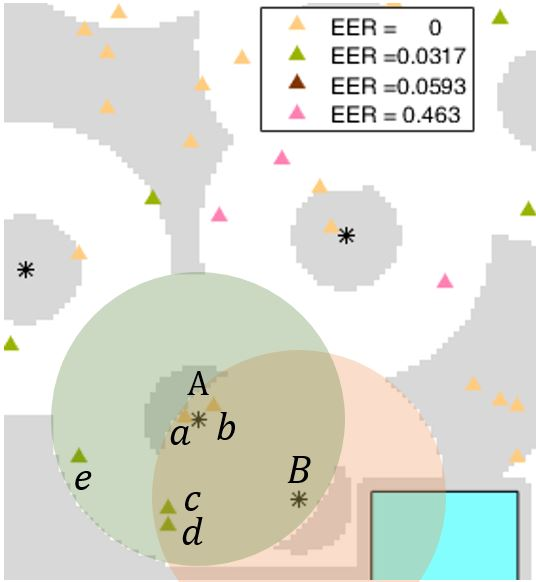
\includegraphics[width=8cm]{figures/EER_zoom}
  \caption{Zoom in of an example of milestones, where the green and orange circles represent the regions that the target A and B can be observed correspondingly. a-e are the generated milestones.}
  \label{fig:17}
\end{figure}


\begin{figure}
 \centering
  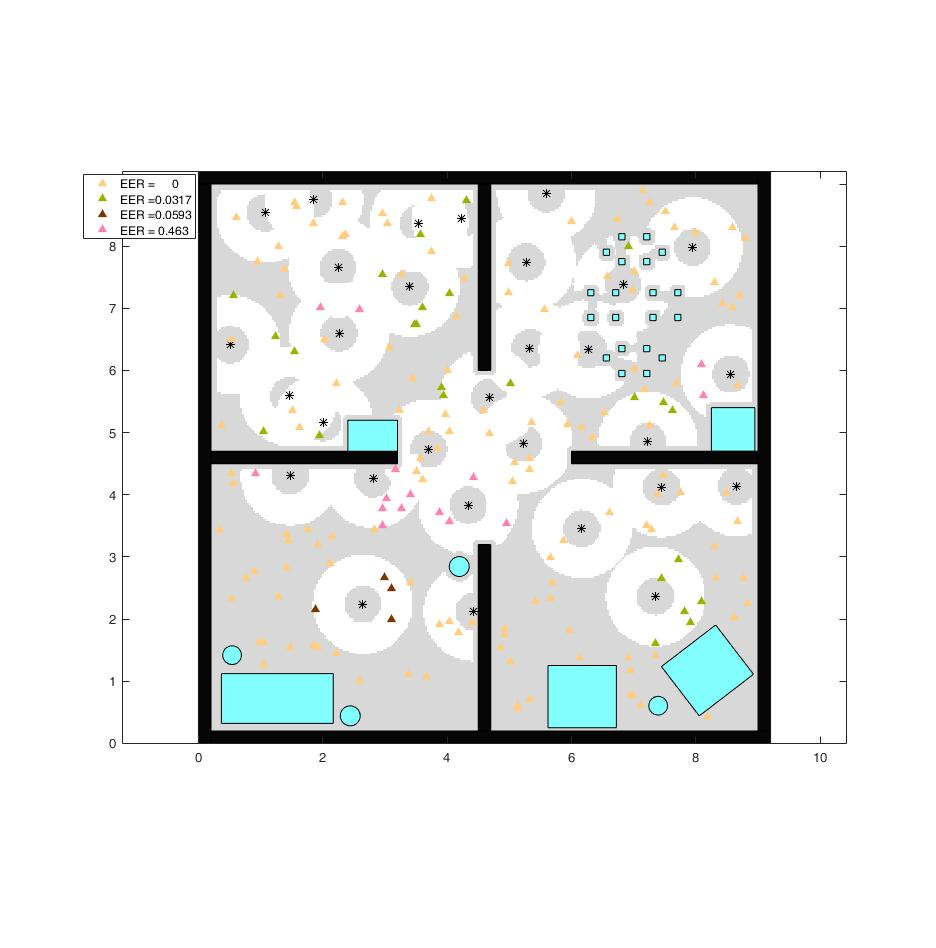
\includegraphics[width=20cm]{figures/milestone180}
  \caption{Example of sampling 180 milestones}
  \label{fig:16}
\end{figure}

\end{document}
